\documentclass[class=article,border=0mm,tikz=true,10pt]{standalone}
\usepackage{graphicx}
\usepackage[group-digits=integer,separate-uncertainty,per-mode=symbol]{siunitx}
\usepackage{xcolor}
\newcommand{\ESTOA}{\frac{S_0}{4}}

\usetikzlibrary {decorations.pathmorphing,positioning}
\begin{document}
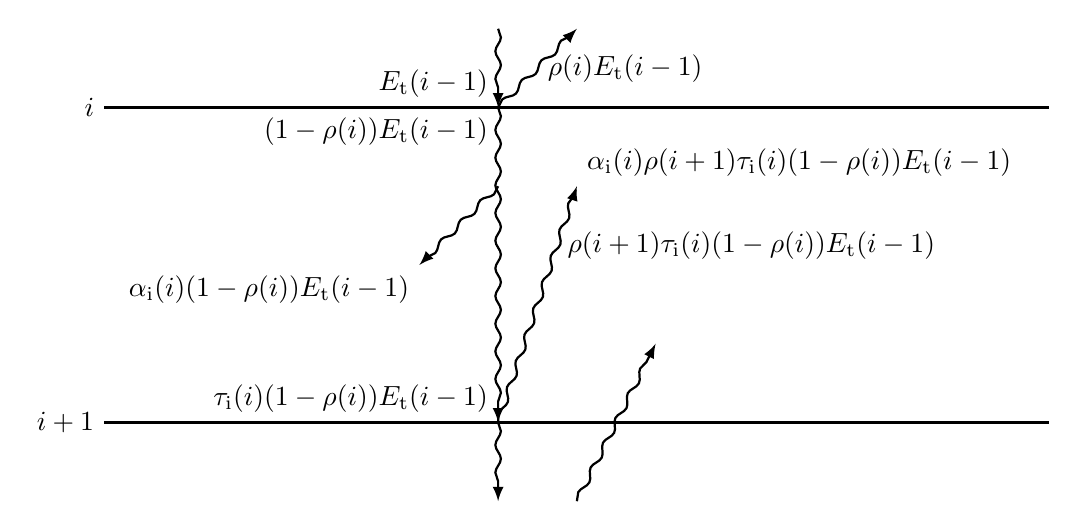
\begin{tikzpicture}[
  thick,
  radiation/.style={
    -latex,
    decorate,
    decoration={
      snake,
      amplitude=1,
      post length=1mm
    }
  }
]
  \draw[radiation] (5,5) -- (5,4)
    node[anchor=south east] {$E_\text{t}(i - 1)$};
  \draw[radiation] (5,4) -- (6,5)
    node[midway,anchor=west] {$\rho(i) E_\text{t}(i - 1)$};
  \draw (0,4)
    node[anchor=east] {$i$}
    -- (12,4);
  \draw[radiation] (5,4)
    node[anchor=north east] {$(1 - \rho(i)) E_\text{t}(i - 1)$}
    -- (5,0)
    node[anchor=south east] {$\tau_\text{i}(i) (1 - \rho(i)) E_\text{t}(i - 1)$};
  \draw[radiation] (5,3) -- (4,2)
    node[anchor=north east] {$\alpha_\text{i}(i) (1 - \rho(i)) E_\text{t}(i - 1)$};
  \draw[radiation] (5,0) -- (6,3)
    node[anchor=south west] {$\alpha_\text{i}(i) \rho(i + 1) \tau_\text{i}(i) (1 - \rho(i)) E_\text{t}(i - 1)$}
    node[near end,anchor=west] {$\rho(i + 1) \tau_\text{i}(i) (1 - \rho(i)) E_\text{t}(i - 1)$};
  \draw (0,0)
    node[anchor=east] {$i + 1$}
    -- (12,0);
  \draw[radiation] (5,0) -- (5,-1);
  \draw[radiation] (6,-1) -- (7,1)
    node[anchor=west] {};
\end{tikzpicture}
\end{document}
